\documentclass[a4paper,10pt]{article}
\usepackage[margin=20mm]{geometry}
\usepackage{graphicx}
\title{SPB Module: EPC2361 Loss and Water-Cooling Screening}
\author{LossCalculation-SPB}
\begin{document}
\maketitle
\section{Which losses are included?}
\subsection{Conduction loss}
An enhanced GaN channel behaves approximately as a resistance. Its instantaneous
loss is $i^2R_{DS(on)}$, so RMS current must be used when averaging. In a
balanced three-phase inverter with $N$ ideally sharing devices per position,
the total is $3I_{phase,rms}^2R_{DS(on)}(T)/N$, with ripple added in quadrature.
The device is warmer in operation than the 25 C datasheet test, and the model
must account for this resistance increase. Unequal sharing and dynamic
on-resistance can increase actual loss beyond this estimate.

\subsection{Switching loss: overlap and output capacitance}
During turn-on and turn-off, nonzero drain voltage and current coexist.
Their overlap produces dissipation. A triangular estimate is
$E_{overlap}\simeq V_{dc}|I|(t_{on}+t_{off})/2$. The assumed overlap intervals
are not the gate-driver command rise/fall time or propagation delay.
The EPC2361 datasheet does not tabulate $E_{on}$ and $E_{off}$ for the intended
current, voltage, resistance, temperature and layout; consequently the initial
analytical calculation uses assumed 5 ns intervals rather than measured energies.

Output capacitance is nonlinear. The stored energy is
\[E_{oss}(V)=\int_0^V v C_{oss}(v)\,dv,\]
not generally $C_{oss}(V)V^2/2$ using the single-point capacitance.
Use the energy curve in Figure 6, or the energy-equivalent capacitance at its
specified voltage. The analytical complementary-device fraction is an adjustable
energy allowance, not a proven commutation-loss partition. Circuit conditions
determine how much stored energy is recovered or dissipated.
Once calibrated switching energies replace this approximation, remove the
overlap/Coss terms already contained in those energies.

\subsection{Deadtime: reverse channel conduction}
During deadtime both gate commands are off, but inductive current must continue.
An enhancement-mode GaN device conducts in its third quadrant, with a reverse
voltage drop that depends on current, temperature and off-state gate voltage.
This plays the freewheeling role often associated with a MOSFET body diode,
but EPC2361 has no silicon-style PN body diode and its datasheet lists zero
reverse-recovery charge. Zero $Q_{rr}$ does not mean zero deadtime or capacitive loss.
For two deadtime intervals per leg per carrier cycle,
$P_{dead}\simeq 6f_s t_d V_{SD}\overline{|I_{phase}|}$ across three legs.
The 2 V reverse drop is an explicit first estimate; it must be replaced with a
reading of Figure 8 at the actual per-device current, or a validated simulation.

\subsection{Gate drive and remaining module losses}
The gate supply delivers approximately $Q_gV_g$ per switching cycle per device,
giving $6NQ_gV_gf_s$. This is dissipated across driver/gate resistances, and is
not all heat in the transistor junction. The model counts it in efficiency but
does not apply it to the transistor cold plate. PCB/copper, capacitors, driver
quiescent power, control and auxiliaries require a separate loss allocation.

\section{Where the parameters come from}
The supplied datasheet is revision 2.4, 20 July 2026. Values below explain the
default configuration; the input JSON and saved summary record the actual run.
\begin{center}\small
\begin{tabular}{p{0.21\linewidth}p{0.32\linewidth}p{0.37\linewidth}}
Parameter & Datasheet source & Treatment in the model \\
\hline
$R_{DS(on)}$ & Page 1: 0.75 mOhm typical, 1 mOhm maximum at 25 C, 5 V gate, 50 A &
Use 1 mOhm and about 1.65 temperature factor at 125 C from Figure 9. Factor is a typical visual reading. \\
$Q_g$, $R_g$ & Page 2: 28 nC typical, 34 nC maximum at 50 V; internal $R_g=0.4$ ohm &
Analytical gate power uses 34 nC. SPICE includes internal gate resistance; external and driver resistance are added once. \\
$E_{oss}$ & Page 3, Figure 6; page 2 $C_{oss,ER}=1419$ pF over 0--50 V &
About 3.2 microjoule visually at 75 V; 50 V value is about 1.77 microjoule. Do not scale constant capacitance blindly to other voltages. \\
$V_{SD}$ & Page 1: 1.6 V at only 0.5 A; Figure 8 provides reverse-current curves &
The 0.5 A point is not a high-current drop. Default 2 V is an assumption pending calibration. \\
$E_{on}$, $E_{off}$ & No matching energy tables; page 6 switching traces use a particular driver and layout &
Initial overlap times are assumed; the separate double-pulse sweep extracts explicitly defined model energies. \\
$R_{jc}$, temperature & Page 1: 0.2 K/W typical to top case, 150 C absolute limit &
Use your 125 C design ceiling; TIM and cold plate are separate assumed resistances. \\
Parasitics and driver & Not specified for the user's PCB &
Sweep loop inductance and external gate resistance. Replace driver impedance and layout assumptions with real data. \\
\end{tabular}
\end{center}
\clearpage

\section{Scope and inputs}
One two-level three-phase inverter module. The 1200 V, 300 kW system is
context only; interconnection and hydraulic arrangement are not modeled.
Continuous SVM uses $V_{phase,pk}=mV_{dc}/2$. All inputs and device values
are saved with this run in results/summary.json.
\begin{center}\begin{tabular}{lr}
@INPUTS@
\end{tabular}\end{center}
Here ambient means local cooling water, sink-to-ambient means shared
cold-plate-to-water resistance, and case-to-sink means individual TIM resistance.
The EPC2361 absolute junction limit is 150 C; its 133 A continuous rating
is specified below 125 C. Neither rating establishes PCB current capability.
The user's design ceiling is 125 C. At 18.75 kW, strictly exceeding 99.5\%
requires less than 94.22 W total module loss.
\section{Loss model}
For balanced sinusoidal currents:
\[V_{phase,rms}=mV_{dc}/(2\sqrt{2}),\qquad
I_{rms}=P_o/(3V_{phase,rms}\cos\phi),\qquad
\overline{|I|}=2\sqrt{2}I_{rms}/\pi.\]
$N$ means devices per switch position: the module contains $6N$ devices.
Conduction loss is
\[P_{cond}=3(I_{rms}^2+I_{ripple,rms}^2)R_{hot}/N.\]
The maximum 25 C resistance is scaled by an approximate typical temperature
factor evaluated at the design limit, rather than iterating temperature.

One hard commutation per leg per carrier cycle gives overlap loss
$3V_{dc}\overline{|I|}(t_{on}+t_{off})f_s/2$.
Capacitance loss allowance is $3NE_{oss}(1+k)f_s$, where $k$ is an adjustable
complementary-device fraction. This is not a commutation simulation.
Gate power is $6NQ_gV_gf_s$; deadtime loss is $6t_dV_{SD}\overline{|I|}f_s$.
Do not add measured total switching energy on top of overlap and capacitance terms.
\section{Cooling model}
Each device has its own junction-to-top-case and TIM branch, then all devices
share one isothermal cold plate. Datasheet typical $R_{jc}=0.2$ K/W.
With hottest-device loss allowance $P_{hot}$:
\[
T_j=T_{water}+P_{FET,total}R_{plate-water}+P_{hot}(R_{jc}+R_{TIM}).
\]
Maximum plate-to-water resistance is
$(T_{j,limit}-T_{water}-P_{hot}(R_{jc}+R_{TIM}))/P_{FET,total}$.
A negative value means the local branch alone is insufficient.
Gate-driver and other losses are outside this plate. Board heat flow, coolant
rise along a channel and transient thermal impedance are excluded.
The exposed top is at source potential; a common half-bridge cold plate
requires an electrically isolating TIM.
\section{Results}
@COUNT@ of @TOTAL@ points pass the modeled constraints. @RESULT@
\clearpage
\begin{center}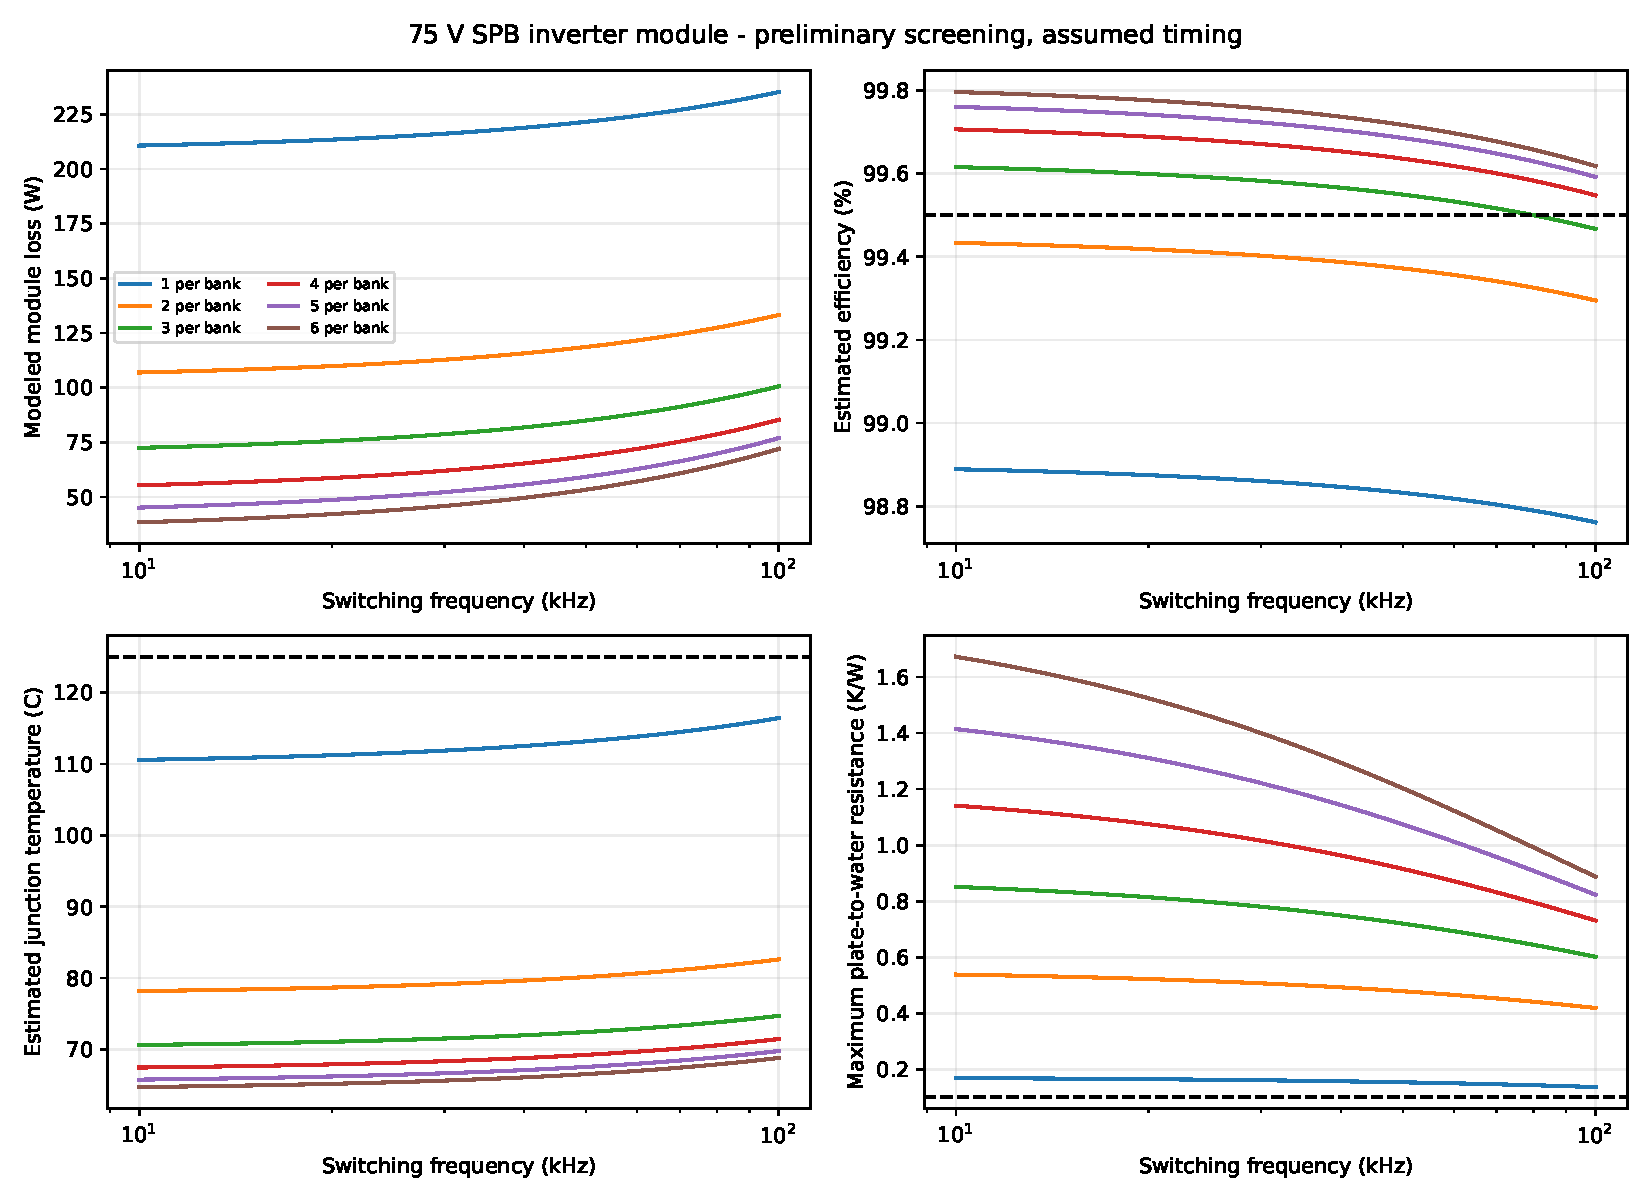
\includegraphics[width=\linewidth]{../../results/sweep.pdf}\end{center}
\section{Interpretation}
CSV outputs contain component losses, current, junction temperature, remaining
loss budget, required cooling resistance and failure reasons. The summary
also records minimum passing parallel count per sampled frequency.

Near the maximum SVM reference, a conservative pulse screen requires
$(1-\sqrt{3}m/2)/(2f_s)>t_d+t_{pulse,min}$.
This assumes centered continuous SVM without pulse suppression; confirm the
actual controller behavior. More parallel devices cannot resolve this limit.

Power factor, phase ripple, overlap times, driver capability, sharing,
overshoot, pulse width, TIM and plate resistance need confirmation.
Zero other losses does not demonstrate full-module efficiency. PCB, capacitor,
control, driver quiescent and auxiliary losses consume the remaining budget.
Ripple inputs affect conduction and peak-current checks; switching ripple
correlations are not modeled. Switching times are assumed fixed as N increases.

Source: supplied EPC2361 datasheet revision 2.4, 20 July 2026, pages 1--3 and 5.
At 75 V, $E_{oss}\approx3.2$ microjoule and the resistance multiplier at 125 C
is about 1.65: visual curve estimates, not guaranteed values. Maximum gate
charge is characterized at 50 V and approximated at 75 V. The model does not
verify dynamic on-resistance, transient SOA, parasitics or switching imbalance.
\end{document}
